\section{Durchführung}
\label{sec:Durchführung}

% Was wurde gemessen bzw. welche Größen wurden variiert?

\begin{figure}
    \centering
    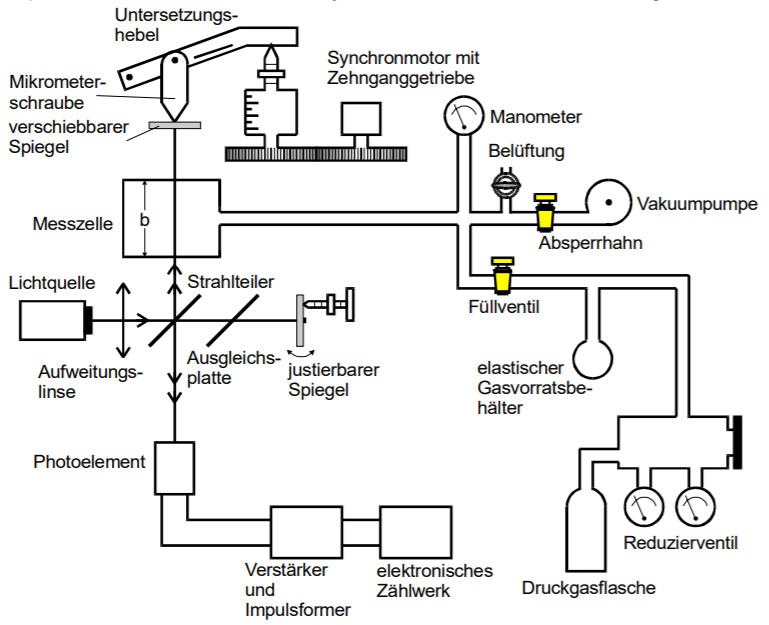
\includegraphics[width=0.4\textwidth]{images/bild4.png}
    \caption{Versuchsaufbau der gesamten Messapperatur.\cite{V401}}
    \label{fig:bild4}
\end{figure}

Zu Beginn der Messung müssen die Spiegel und der Laser aufeinander abgestimmt werden. 
Auf dem Photoelement, also dem Detektor, werden dazu die beiden hellsten Reflektionen gesucht und über Verschieben des Lasers bzw. des justierbaren Spiegels übereinander gebracht.
Außerdem wird die Höhe des Photoelements so eingestellt, dass die Strahlen des Lasers auf den Eintrittsspalt treten.

Der andere justierbare Spiegel kann über eine Schraube, die von einem Motor angetrieben wird, präzise verschoben werden.
Auf der Schraube ist außerdem eine Angabe über die Größe der Verschiebung zu finden.
Vor der Messung wird die Schraube auf einen möglichst genauen Wert eingestellt.
Zudem wird die Hebelübersetzung notiert, die auf dem Gerät angegeben ist. 

Der Motor wird in einer Geschwindigkeit betrieben, in der alle Impulse vom Zählwerk erfasst werden können. 
Nach etwa 3000 gemessenen Interferenzen wird die Messung gestoppt und der Wert für $d$ wird notiert. 
Diese Messung wird zehn mal durchgeführt.

Für den zweiten Teil der Messung wird die Messzelle auf den Druck $p'$ evakuiert. 
Dieser Wert wird notiert.
Dann wird der Druck langsam wieder normalisiert, in dieser Zeit werden Interferenzen gezählt.
Der Druck der sich danach einstellt, wird als $p_0$ ebenfalls notiert.
Diese Messung wird fünf mal durchgeführt.